%!TeX root = ../main.tex
\section{Esparcimiento, extinción y absorción}

En la sección anterior, se estudió cómo se relaciona el campo eléctrico que incide en una partícula arbitraria con el campo eléctrico esparcido por esta, dando como resultado la relación de la Ec. \eqref{eq:MEsparcimientoGral}. En esta sección, se estudia el balance de energía al presentarse el fenómeno de esparcimiento.

Supóngase un haz de luz cruza por un medio donde se encuentran partículas arbitrarias (ver Fig. \ref{fig:EnergiaDetector}) y que la energía medida por un detector colocado detrás de las partículas  es $U$. En el caso donde no hubiera partículas, la energía que mediría el detector sería $U_0$ , con $U_0 > U$.  La diferencia de energía $U_0-U$ entre ambos casos es atribuida tanto a la absorción de las partículas (conversión de la energía EM en otras formas de energía, como calor), como al esparcimiento de la luz en direcciones distintas a la posición del detector. Al efecto en conjunto de la absorción y del esparcimiento se denomina extinción.

	\begin{figure}[h!]\centering
%	\tdplotsetmaincoords{60}{110}
%	\pgfmathsetmacro{\rvec}{1. 3}
%	\pgfmathsetmacro{\thetavec}{30}
%	\pgfmathsetmacro{\varphivec}{60}
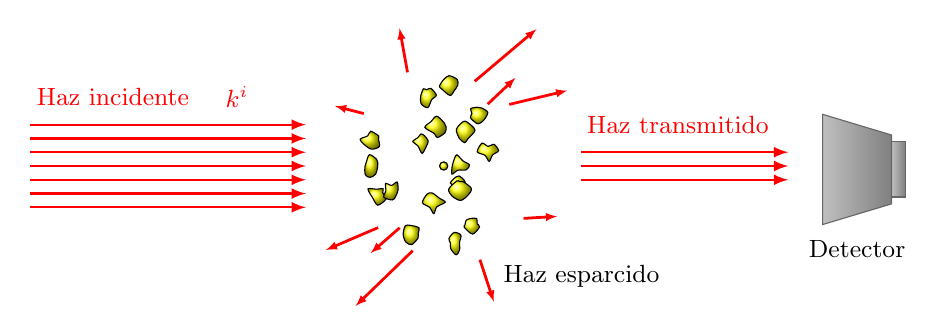
\begin{tikzpicture}[scale=3.5]
\def\d{.75}

%------- Scatterers cloud
\foreach \i in {0,20,40,60,...,360}{
\pgfmathsetseed{\i}
\draw[ball color=yellow, opacity = 1,scale =.03,rotate = rnd, shift={({10*rnd*cos(\i)},{10*rnd*sin(\i)})}]
	 plot [smooth cycle, samples=8,domain={1:8}]
     (\x*360/8+5*rnd:0.5cm+1cm*rnd) node at (0,0) {};
}
%------ Incident wave
	\foreach \i in {-3,...,3}{
		\draw[thick,red, - latex] (-1.5,\i/20)--(-.5,\i/20);}
	\node at (-1.2,5/20){\small \color{red}Haz incidente};	
	\node at (-.75, 5/20) {\small \color{red}$\vb{k}^i$};
%------ Transmitted wave	
	\foreach \i in {-1,...,1}{
\draw[thick,red, - latex] (.5,\i/20)--(1.25,\i/20);}
\node at (.85,3/20){\small \color{red}Haz transmitido};	

%------- Detector
\node at ( 1.5, -6/20){\small Detector};
\begin{scope}[scale  = .25, shift = {(3.5,-2.3)}, rotate = 90, shift = {(-.25,-5)}]
\shade[left color=gray!50!white,right color=gray] (1.7,3)
    -- ++(1.6,0) -- ++(-0.3,-1) -- ++(-1,0) -- cycle;% column
  \shade[left color=gray!50!white,right color=gray] (2.1,2)
    -- ++(0.8,0) -- ++(0,-0.2) -- ++(-0.8,0) -- cycle;% column bottom
  \draw[gray!80!black] (1.7,3) -- ++(1.6,0) -- ++(-0.3,-1)
    -- ++(-1,0) -- cycle;%column
  \draw[gray!80!black] (2.1,2) -- ++(0,-0.2) -- ++(0.8,0)
    -- ++(0,0.2);%column bottom
\end{scope}	

%------- Campo esparcido
\node at ( .5, -8/20){\small Haz esparcido};
\begin{scope}[opacity=1, transparency group, scale = .15]
\foreach \s in {-1,1}{
	\draw[- latex, red](0,\s*\d)++(25:\s*1.75)--(35+rand*5:\s*3.5);
	\draw[- latex, red](0,\s*\d)++(35:\s*1.3)--(55+rand*5:\s*2.75);
	\draw[- latex, red](0,\s*\d)++(165:\s*2)--(155+rand*5:\s*3);
	\draw[- latex, red](0,\s*\d)++(120:\s*1.75)--(110+rand*5:\s*3.5);
	\draw[- latex, red](0,\s*\d)++(60:\s*1.5)--(60+rand*5:\s*4);}
\end{scope}

\end{tikzpicture}
%
\caption{Diagrama de la extinción de luz por una nube de partículas esparcidoras. La energía que mide el detector en la ausencia de partículas es $U_0$ sin embargo, al interactuar la luz con las partículas, la lectura de energía es $U$. La energía $U-U_0$  corresponde a la energía que no llega al detector asociada tanto al esparcimiento de luz, como a la absorbida por las partículas; al conjunto de estos fenómenos se le denomina extinción.}\label{fig:EnergiaDetector}
	\end{figure}	
	
Ahora, considérese el caso de una sola partícula (de tamaño  forma arbitraria) inmersa en un medio dispersor e iluminada por una onda plana; debido a la onda plana, la partícula esparce luz.  Para cuantificar la energía esparcida por la partícula, defínase una esfera $A$ de radio $r$ que contenga a la partícula. La energía total  por unidad de tiempo que cruza la superfice de $A$ se calcula como
%
\begin{align}
W_{abs} = -\int_A \ev{\vb{S}}_t\cdot \vu{e}_r \dd{a},
\label{eq:Wa}
\end{align}
%
donde $\ev{\cdot}_t$ denota el promedio temporal, y donde el vector de Poyntig $\vb{S}$ puede descomponerse en tres contribuciones:
%
\begin{align}
\ev{\vb{S}}_t &= \frac12 \Re[\vb{E}\times\vb{H}^*] = \ev{\vb{S}^i}_t + \ev{\vb{S}^{sca}}_t + \ev{\vb{S}^{ext}}_t,
\label{eq:PoyntingContribuciones}\\
\ev{\vb{S}^i}_t &= \frac12 \Re[\vb{E}^i\times\vb{H}^{*i}], \\
\ev{ \vb{S}^{sca}}_t &= \frac12 \Re[\vb{E}^{sca}\times\vb{H}^{sca*}] ,\\
\ev{\vb{S}^{ext}}_t &= \frac12 \Re[\vb{E}^i\times\vb{H}^{sca*} + \vb{E}^{sca} \times\vb{H}^{i*}],
\label{eq:Sext}
\end{align}
%
siendo $i$ y $sca$ los subíndices que denotan a los campos EMs incidentes y esparcidos (\textit{scattering} en inglés), respectivamente, mientras que $ext$ corresponde al campo EMs resultado de la interferencia entre la onda incidente y los campos esparcidos; a este término lo asociaremos a la extinción.

Según la Ec \eqref{eq:Wa}, si $W_{abs}>0$ entonces la energía es absorbida dentro de la esfera, y si $W_{abs}<0$ entonces energía es generada en la partícula, aunque a lo largo de este texto se excluye este caso. Al descomponer a $W_{abs}$ en las mismas contribuciones que al  vector de Poynting en la Ec. \eqref{eq:PoyntingContribuciones}, obtenemos que
%
\begin{align}
W_{abs} &= W_i - W_{sca} + W_{ext},
\end{align}
%
con
%
\begin{align}
W_{i} &= -\int_A\ev{\vb{S}^i}_t\cdot \vu{e}_r \dd{a} = 0,\\
W_{sca} &= \int_A\ev{\vb{S}^{sca}}_t\cdot \vu{e}_r \dd{a},\label{eq:Wsca}\\
W_{ext} &= -\int_A\ev{\vb{S}^{ext}}_t\cdot \vu{e}_r \dd{a},
\end{align}

donde $W^i=0$ dado que la partícula se encuentra en un medio no disipativo. Es decir, que la energía extinta por unidad de tiempo es
%
\begin{align}
W_{ext} = W_{abs} + W_s,
\end{align}
%
como se describió al inicio de esta sección.	

Como caso particular, supóngase que la onda plana incidente está polarizada en la dirección $x$, es decir que $\vb{E}^i = E_0\vu{e}_x$, con $E_0$	 la amplitud del campo eléctrico incidente. Empleando la  expresión para el campo eléctrico esparcido $\vb{E}^{sca}$ como función del campo incidente [Ec. \eqref{eq:MEsparcimientoGral}] y empleando la Ec. \eqref{eq:EIncidenteFull}, así como la ley de Faraday-Lenz, los campos EMs esparcidos se escriben como
%
\begin{align}
\vb{E}^{sca}(\vb{r}) &= \frac{e^{ik(r-z)}}{-ikr}E_0\vb{X}(\theta,\varphi),
\label{eq:EscaX}\\
\vb{H}^{sca}(\vb{r}) &= \frac{e^{ik(r-z)}}{kr\omega\mu}E_0\vu{e}_r\times\vb{X}(\theta,\varphi),
\label{eq:HscaX}
\end{align}
%
con $\vb{X}\cdot\vu{e}_r = 0$ dada por
%
\begin{align}
\vb{X}(\theta,\varphi) = (S_2\cos\varphi + S_3\sin\varphi)\vu{e}_{\parallel}^{s} + (S_4\cos\varphi + S_1\sin\varphi)\vu{e}_{\perp}^{s},
\end{align}
%
donde $S_j = S_j(\theta,\varphi)$.

Para calcular la energía por unidad de tiempo $W_{ext}$ asociada a la extinción que cruza a una superficie esférica $A$ de radio $r$, se emplean las Ecs. \eqref{eq:Sext}, \eqref{eq:EscaX} y \eqref{eq:HscaX}  (\ref{ex:Wext}), dando como resultado que
%	
\begin{align}
W_{ext} &= -\int_{A} \ev{\vb{S}^{ext}}_t\cdot\vu{e}_r\dd{a}\notag\\
 &= \frac{kE_0^2}{2\mu\omega}\Re\bigg\{
\frac{e^{-ikr}}{-ikr}
	\int_A e^{ikz} (\vu{e}_x\cdot\vb{X}^*)\dd{a}\notag\\
&\qquad\qquad+\frac{e^{ikr}}{ikr}
	\int_A e^{-ikz}(\vb{X}\cdot\vu{e}_x)\cos\theta\dd{a}\notag\\
&\qquad\qquad-\frac{e^{ikr}}{ikr}
	\int_A e^{-ikz}(\vb{X}\cdot\vu{e}_z)\sin\theta\cos\varphi\dd{a}
	\bigg\},
	\label{eq:WextX}
\end{align}
donde $ikz = ikr\cos\theta$ y $\dd{a} =r^2 \sin\dd{\theta}\dd{\varphi}$. Para resolver las integrales de la Ec. \eqref{eq:WextX}, empleemos dos veces la integración por partes el siguiente caso general con $\mu = \cos\theta$ 
%
\begin{align}
\int_{-1}^{1} e^{\pm ikr\mu}f(\mu)\dd{\mu} = \pm
f(\mu)\frac{e^{\pm ikr\mu}}{ikr}\eval_{-1}^1 -
\frac{\mp 1}{(kr)^2}\qty(
\dv{f(\mu)}{\mu}e^{\pm ikr\mu}\eval_{-1}^1 -\int_{-1}^1\dv[2]{f(\mu)}{\mu}e^{\pm ikr\mu}\dd{\mu}
).
\label{eq:eikmu}
\end{align}
%
Dado que consideramos una región del espacio tal que $kr\gg 1$, la expresión de la Ec. \eqref{eq:eikmu} se aproxima a
%
\begin{align}
\int_{-1}^{1} e^{\pm ikr\mu}f(\mu)\dd{\mu} \approx \frac{\pm 1}{ikr}\qty(f(1) e^{\pm ikr} - f(-1)e^{\mp ikr}).
\label{eq:approxInt}
\end{align}
%
Escogiendo $f_1(\mu) = 1, f_2(\mu) = \mu$ y $f_3(\mu) = \sqrt{1-\mu^2}$ para los integrandos de la Ec. \eqref{eq:WextX} y empleando la aproximación de la Ec. \eqref{eq:approxInt}, vemos que la integral con el término $f_3$ se anula, por lo que la única contribución es\footnote{Al escribir $\vb{X}$ en la base cartesiana canónica, esta cantidad no depende de $\varphi$, por lo que la integral en esta variable es $2\pi$.}
%
\begin{align}
W_{ext} &=  \frac{2\pi kE_0^2}{2\mu\omega k^2}\Re\bigg\{
e^{-ikr}\qty[
 e^{ikr} (\vu{e}_x\cdot\vb{X}^*) \eval_{\theta=0} - e^{-ikr} (\vu{e}_x\cdot\vb{X}^*) \eval_{\theta=\pi}
 ] \notag \\
&\qquad\qquad\qquad+e^{ikr}\qty[
 e^{-ikr}(\vb{X}\cdot\vu{e}_x)\eval_{\theta=0} + e^{ikr}(\vb{X}\cdot\vu{e}_x)\eval_{\theta = \pi}
	 ]
	\bigg\},\\
	&=  \frac{2\pi kE_0^2}{2\mu\omega k^2}\Re\bigg\{
\qty[
(\vb{X}\cdot\vu{e}_x)\eval_{\theta=0} +
 (\vu{e}_x\cdot\vb{X}^*) \eval_{\theta=0} 
 ]\notag \\
&\qquad\qquad\qquad+\qty[e^{2ikr}(\vb{X}\cdot\vu{e}_x)\eval_{\theta = \pi} - e^{-2ikr} (\vu{e}_x\cdot\vb{X}^*) \eval_{\theta=\pi}
	 ]
	\bigg\}.
\end{align}
%
Los términos entre paréntesis pueden reescribirse como $2\Re\{\vb{X}\cdot\vu{e}_x\}$, evaluado en $\theta = 0$, y $2i\Im\{e^{2ikr}(\vb{X}\cdot\vu{e}_x)\}$	, evaluado en $\theta = \pi$, por lo que al calcular la parte real, concluimos que la energía  asociada a la extinción  por unidad de tiempo que cruza una superficie esférica es
%
\begin{align}
W_{ext} = \qty(\frac{kE_0^2}{2\mu\omega})\frac{4\pi}{k^2} \Re\qty[(\vb{X}\cdot\vu{e}_x)\eval_{\theta = 0 }] = I_i \frac{4\pi}{k^2}\Re\qty[(\vb{X}\cdot\vu{e}_x)\eval_{\theta = 0 }],
\label{eq:WextXFull}
\end{align}
% 
donde $I_i$ es la irradiancia (energía por unidad de tiempo por unidad de área) de la onda plana incidente. El término que multiplica a $I_i$ en la Ec. \eqref{eq:WextXFull} tiene unidades de área y se le conoce como la sección transversal de extinción, dada por la expresión
%
\begin{align}
C_{ext,x} = \frac{4\pi}{k^2}\Re\qty[(\vb{X}\cdot\vu{e}_x)\eval_{\theta = 0 }],
\label{eq:Cextx}
\end{align}
%
con el subíndice $x$ denotando explícitamente la polarización de la onda plana incidente. Se forma semejante, se definen las secciones transversales de absorción $C_{abs} = W_{abs}/I_i$ y de esparcimiento $C_s = W_s/I_i$, que se relacionan por medio de la Ec.  \eqref{eq:Wa} cumpliendo que
%
\begin{align}
C_{ext} = C_{abs} + C_{sca}.
\label{eq:C-All}
\end{align}
%

Para obtener una expresión de $C_{sca}$, calculemos  $W_{sca}$ [Ec. \eqref{eq:Wsca}] con los campos EMs esparcidos [Ecs. \eqref{eq:EscaX} y \eqref{eq:HscaX}] considerando, nuevamente, una onda plana incidente polarizada en la dirección $x$. Al dividir $W_{sca}$ por la irradiancia de una onpla plana, obtenemos que
%
\begin{align}
C_{sca,x} &=  \int_A \frac{\vb{X}\cdot\vb{X}^*}{(kr)^2}\vb{e}_r\cdot\vb{e}_r\dd{a} = \int_{4\pi}\frac{\norm{\vb{X}}^2}{k^2}\dd{\Omega},
 \label{eq:Cscax}
\end{align}
%
donde $\dd{\Omega} = \sin\theta\dd{\theta}\dd{\varphi}$ es el diferencial de ángulo sólido y el $4\pi$ en el símbolo de la integral denota que se realiza la integral en toda la esfera. El integrando de la Ec. \eqref{eq:Cscax}, denominado sección transversal diferencial de esparcimiento y denotado simbólicamente como $\dv*{C_{sca}}{\Omega}$, define la distribución angular de luz esparcida, por unidad de irradiancia. en una unidad de ángulo sólido, en una dirección específica \cite{bohren1998absorption}.

Asimismo, existe una relación multiplicativa entre la distribución angular de la luz esparcida y la sección transversal de esparcimiento de la partícula. Ésta es conocida como la función de fase $p$ –o bien diagrama de esparcimiento– 
%
\begin{align}
p =  \frac{\norm{\vb{X}}^2}{k^2} C_{sca},\qquad\text{tal que}\qquad \int_{4\pi}p\dd{\Omega} = 1,
\end{align}
%
es decir, $p$ es una función normalizada. Para clasificar el esparcimiento de una partícula según la distribución angular de la luz, se emplea el parámetro de asimetría $g$, dado por
%
\begin{align}
g = \langle \cos\theta \rangle_p  = \int_{4\pi}p\cos\theta\dd{\Omega},
\end{align}
%
que es el promedio de la proyección de la luz esparcida sobre la dirección de propagación de la onda plana incidente. Si la partícula esparce la luz de manera isótropa, el parámetro de asimetría toma el valor de cero; lo mismo ocurre si el esparcimiento es simétrico al rededor del ángulo $\theta = \pi/2$ (es decir, esparce lo mismo hacia delante que hacia atrás. Dado el caso en el que la partícula esparza más luz en la dirección frontal ($\theta = 0$), $g$ toma valores positivos. Por otro lado, un mayor esparcimiento en la dirección posterior ($\theta = \pi$) corresponde a valores negativos de $g$.
	
Todas las expresiones y cálculos desarrollados hasta el momento se realizaron acabo bajo la suposición de luz polarizada en la dirección $x$, sin embargo se pueden generalizar suponiendo una onda plana incidente de la forma $\vb{E}^i = E_x\vu{e}_x + E_y\vu{e}_y$. Para este caso, el campo eléctrico esparcido se escribe según la Ec. \eqref{eq:MEsparcimientoGral} como 
%
\begin{align}
\vb{E}^{sca} = \frac{e^{ik(r-z)}}{-ikz}\qty(E_x\vb{X} + E_y\vb{Y}) =  \frac{e^{ik(r-z)}}{-ikz}\vb{T},
\end{align}
%
donde $\vb{X}$ y $\vb{Y}$ dependen de los coeficientes de la matriz de esparcimiento $\mathbb{S}$. Haciendo los procedimientos análogos a las Ecs. \eqref{eq:Cscax} y \eqref{eq:Cextx}, obtenemos que
%
	\begin{tcolorbox}[title = {Secciones transversales de extinción, absorción y esparcimiento} , ams align ]
C_{ext} &= C_{abs} + C_{sca},
\label{eq:OptTeo}\\
C_{ext} &= \frac{4\pi}{k^2\norm{\vb{E}^i}}\Re\bigg\{(\vb{E}^{i*}\cdot\vb{T})\eval_{\theta = 0} \bigg\},
\label{eq:CextGeneral}\\
C_{sca} &= \int_{4\pi} \frac{\norm{\vb{T}}^2}{k^2\norm{\vb{E}^i}^2}\dd{\Omega}.
\label{eq:CscaGeneral}
	\end{tcolorbox} 
%
Para el caso particular de luz no polarizada, se cumple que
%
\begin{align}
\langle E_xE_x^*\rangle = \langle E_yE_y^*\rangle,
\qquad\mbox{y}\qquad
\langle E_xe_y^*\rangle = \langle E_ye_x^*\rangle = 0,
\end{align}
%
es decir que no hay términos cruzados. Por lo tanto, las expresiones para las secciones transversales de extinción y esparcimiento se pueden dividir en dos componentes, dando como resultado
%
\begin{align}
C_{ext} &=\frac12 \qty(C_{ext,x}+C_{ext,y}),\\
C_{abs} &=\frac12 \qty(C_{abs,x}+C_{abs,y}),
\end{align}
%
donde los subíndices denotan la polarización de la luz esparcida.
	
Para poder comparar la cantidad de luz extinta por partículas de distintos tamaños y formas, se emplean las eficiencias de absorción, esparcimiento y extinción, denotadas por la letra $Q$. Este parámetro se calcula a través de las secciones transversales de absorción, esparcimiento y extinción al normalizarlas por la sección transversal geométrica $C_{geo}$ proyectada en un plano perpendicular a la luz incidente, dando como resultado
%
\begin{align}
\frac{C_{ext}}{C_{geo}} = \frac{C_{abs}}{C_{geo}} + \frac{C_{sca}}{C_{geo}} \quad\longrightarrow \quad
Q_{ext} &= Q_{abs} + Q_{sca}.
\end{align}
%
De manera intuitiva, la eficiencia de extinción $Q_{ext}$ debería ser idéntica a la unidad sin embargo, dicho resultado es válido únicamente en el régimen de la óptica geométrica.{\bf\color{red}Mencionar que esto se estudiará más adelante una vez que  tengamos la solución de Mie??}
	
	
	
	